% floats/figures.tex
% ----------------------------------------------------------------------

% fig:locmap
\begin{figure}[t]
	\vspace*{2mm}
	\begin{center}
		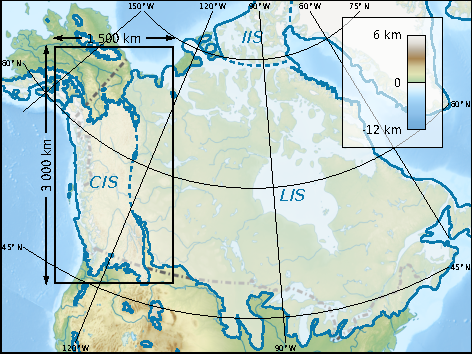
\includegraphics[width=8cm]{cordillera-climate-locmap}
	\end{center}
	\caption{Shaded relief map of northern North America with the extent of the Cordilleran (CIS), Laurentide (LIS) and Innuitian (IIS) ice sheets at 14\,$^{14}$C\,ka\,BP (16.8\,cal\,ka\,BP) \citep{dyke-2004}. While this age denotes the LIS after retreat from its LGM, it closely corresponds to the LGM extent of most of the Cordilleran ice sheet \citep{porter-swanson-1998,dyke-2004,stroeven-etal-2010}. The rectangular box denotes the modelling domain of the Cordilleran ice sheet of 1500 by 3000\,km. Major mountain ranges covered by the ice sheet include the Wrangell and St.-Elias mountains (W-SE), the Selwyn and MacKenzie mountains (S-MK), the Coast Mountains and the Rocky Mountains. The background map consists of ETOPO1 \citep{data:etopo1} and Natural Earth Data \citep{data:naturalearth} and was assembled with GRASS~GIS \citep{soft:grass}.}
	\label{fig:locmap}
\end{figure}

% fig:topo
\begin{figure*}[t]
	\vspace*{2mm}
	\begin{center}
		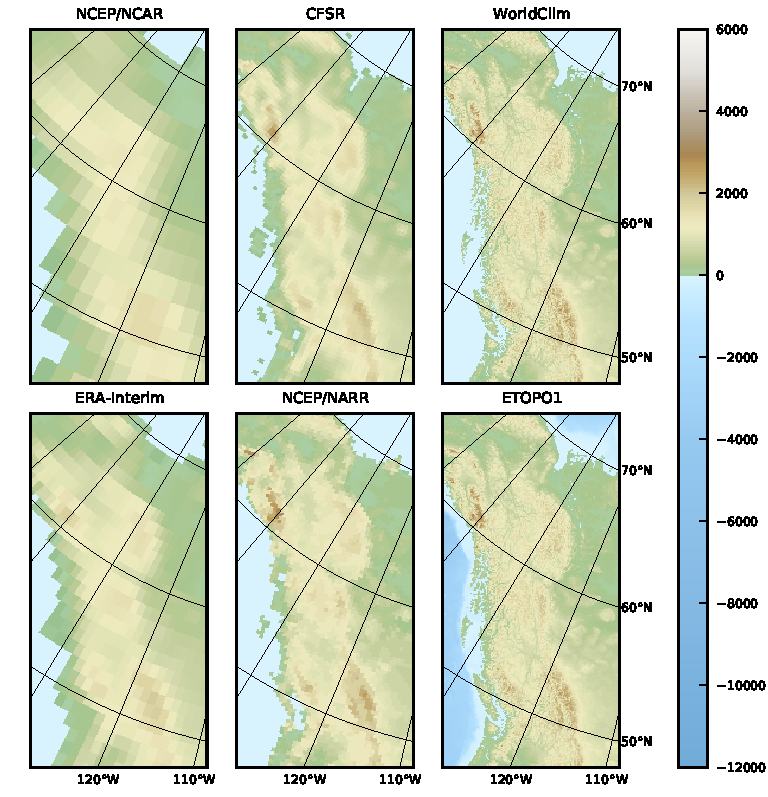
\includegraphics{cordillera-climate-topo}
	\end{center}
	\caption{Topography maps from WorldClim \citep{data:worldclim}, ERA-Interim reanalysis \citep{data:erai}, North American Regional Reanalysis \citep[NARR;][]{data:narr}, ETOPO1 \citep{data:etopo1}, Climate Forecast System Reanalysis \citep[CFSR;][]{data:cfsr}, and NCEP/NCAR reanalysis \citep{data:ncar}. Whereas ETOPO1 is used as basal topography for the ice sheet model, all other data are used as a reference for temperature lapse-rate corrections. Fig.~\ref{fig:topo}-\ref{fig:durationstack} are drawn using Matplotlib \citep{soft:mpl}.}
	\label{fig:topo}
\end{figure*}

% fig:temp
\begin{figure*}[t]
	\vspace*{2mm}
	\begin{center}
		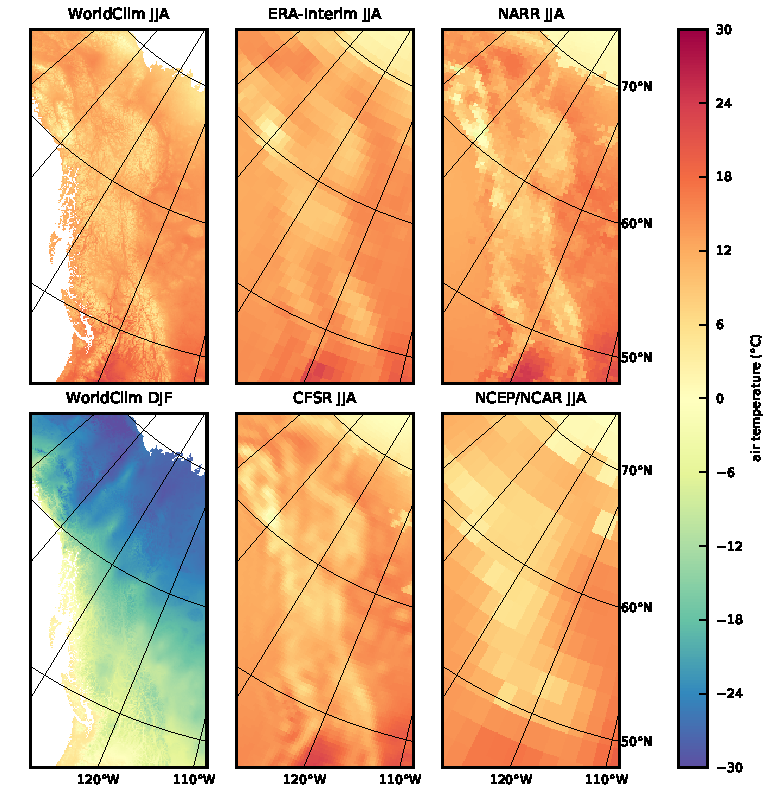
\includegraphics{cordillera-climate-temp}
	\end{center}
	\caption{Summer (JJA) and winter (DJF) temperature maps from WorldClim \citep{data:worldclim}, and summer (JJA) temperature maps from ERA-Interim reanalysis \citep{data:erai}, North American Regional Reanalysis \citep[NARR;][]{data:narr}, Climate Forecast System Reanalysis \citep[CFSR;][]{data:cfsr}, and NCEP/NCAR reanalysis \citep{data:ncar} climatologies.}
	\label{fig:temp}
\end{figure*}

% fig:prec
\begin{figure*}[t]
	\vspace*{2mm}
	\begin{center}
		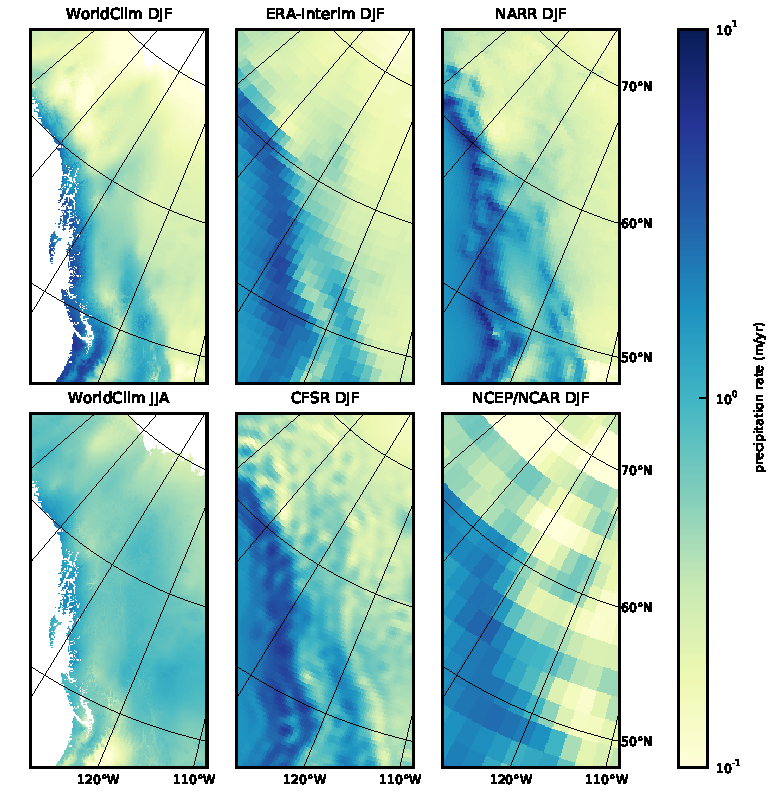
\includegraphics{cordillera-climate-prec}
	\end{center}
	\caption{Winter (DJF) and summer (JJA) precipitation maps from WorldClim \citep{data:worldclim}, and winter (DFJ) temperature maps from ERA-Interim reanalysis \citep{data:erai}, North American Regional Reanalysis \citep[NARR;][]{data:narr}, Climate Forecast System Reanalysis \citep[CFSR;][]{data:cfsr}, and NCEP/NCAR reanalysis \citep{data:ncar} climatologies. Additional forcing data was prepared to correct for wave-like precipitation artefacts in CFSR (section~\ref{sec:climate}).}
	\label{fig:prec}
\end{figure*}

% fig:ivolarea
\begin{figure}[t]
	\vspace*{2mm}
	\begin{center}
		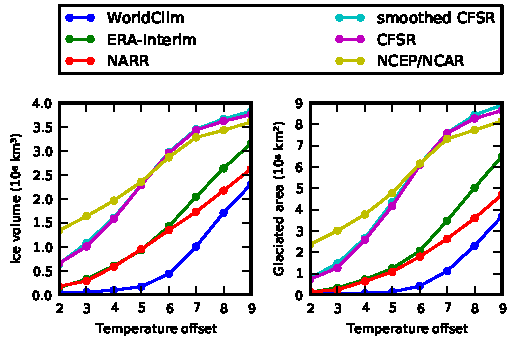
\includegraphics{cordillera-climate-ivolarea}
	\end{center}
	\caption{Total glaciated area and ice volume after 10\,ka as a function of temperature offset for each climate forcing used.}
	\label{fig:ivolarea}
\end{figure}

% fig:extent
\begin{figure*}[t]
	\vspace*{2mm}
	\begin{center}
		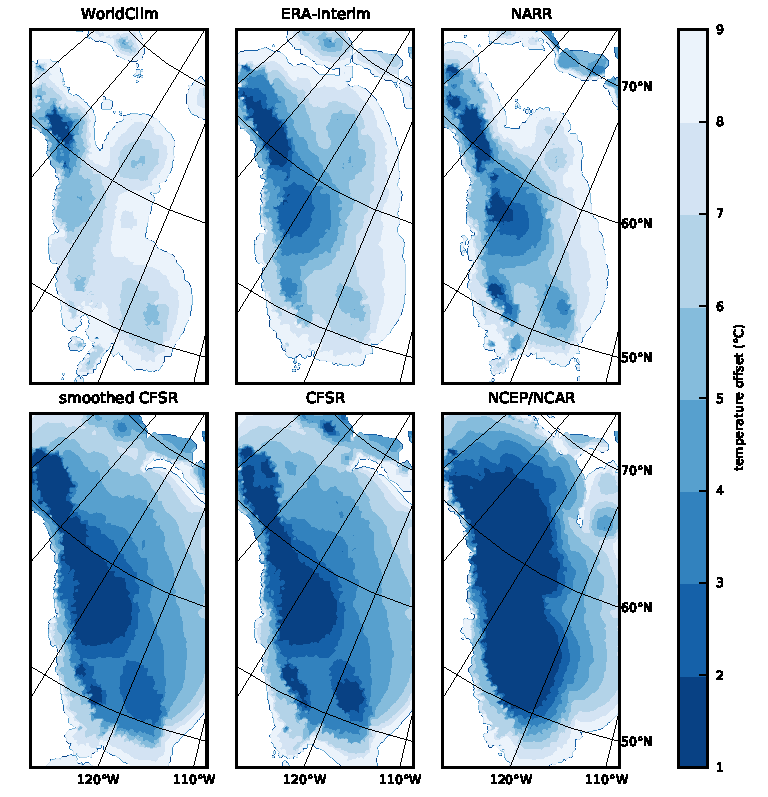
\includegraphics{cordillera-climate-extent}
	\end{center}
	\caption{Extent of ice cover after 10\,ka as a function of applied temperature offsets for each climate forcing used.}
	\label{fig:extent}
\end{figure*}

% fig:cool05
\begin{figure*}[t]
	\vspace*{2mm}
	\begin{center}
		\includegraphics{cordillera-climate-cool05}
	\end{center}
	\caption{Ice surface topography (1 km contours) and velocity (\unit{m\,a^{-1}}) after 10\,ka under a climate 5\,\unit{\degree C} colder than present for each climate forcing used.}
	\label{fig:cool05}
\end{figure*}

% fig:tempheatmap
\begin{figure}[t]
	\vspace*{2mm}
	\begin{center}
		\includegraphics{cordillera-climate-tempheatmap}
	\end{center}
	\caption{Density maps showing a comparison of summer (JJA) surface air temperature data from the WorldClim climatology, against that of each reanalysis. Apparent horizontal lines are an artefact of different horizontal resolutions. Colour mapping is based on a logarythmic scale. Note the cold bias of NCEP/NCAR data relative to WorldClim data.}
	\label{fig:tempheatmap}
\end{figure}

% fig:tempdiff
\begin{figure}[t]
	\vspace*{2mm}
	\begin{center}
		\includegraphics{cordillera-climate-tempdiff}
	\end{center}
	\caption{Summer (JJA) surface air temperature difference maps against WorldClim data, after bi-linear spatial interpolation. Note the cold bias of NCEP/NCAR data and temperature anomalies due to unresolved topographic detail.}
	\label{fig:tempdiff}
\end{figure}

% fig:precheatmap
\begin{figure}[t]
	\vspace*{2mm}
	\begin{center}
		\includegraphics{cordillera-climate-precheatmap}
	\end{center}
	\caption{Density maps showing a comparison of winter (DJF) precipitation rate from the WorldClim climatology, against that of each reanalysis. Apparent horizontal lines are an artefact of different horizontal resolutions. Apparent vertical lines at low values are an artefact of the low precision of WorldClim data. Colour mapping is based on a logarythmic scale. Note the wet bias of all reanalysis data relative to WorldClim data.}
	\label{fig:precheatmap}
\end{figure}

% fig:precdiff
\begin{figure}[t]
	\vspace*{2mm}
	\begin{center}
		\includegraphics{cordillera-climate-precdiff}
	\end{center}
	\caption{Winter (DJF) precipitation rate difference maps against WorldClim data, after bi-linear spatial interpolation. Note the wet bias of all reanalysis data and the large anomalies of CFSR and NCEP/NCAR data.}
	\label{fig:precdiff}
\end{figure}

% fig:oroprecip
\begin{figure}[t]
	\vspace*{2mm}
	\begin{center}
		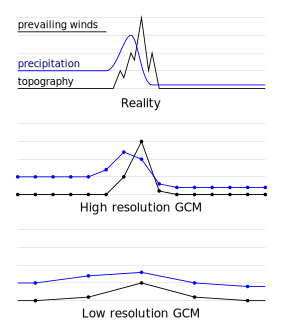
\includegraphics{cordillera-climate-oroprecip}
	\end{center}
	\caption{Schematic representation of the orographic precipitation effect over a mountain range. In a GCM of low resolution, the precipitation peak appears downwind-shifted and smoother and the precipitation shadow is less pronounced than in a high resolution GCM.}
	\label{fig:oroprecip}
\end{figure}

% fig:biatm
\begin{figure*}[t]
	\vspace*{2mm}
	\begin{center}
		\includegraphics{cordillera-climate-biatm}
	\end{center}
	\caption{Ice surface topography (1 km contours) and velocity (\unit{m\,a^{-1}}) after 10\,ka using “hybrid” climate forcing with precipitation rate from WorldClim and surface air temperature from each reanalysis (upper row), and surface air temperature from WorldClim and precipitation rate from each reanalysis (lower row). In other words, the upper row shows the effect of temperature anomalies, and the lower row the effect of precipitation anomalies, for each reanalysis, relative to WorldClim data. Each simulation uses a 5\,\unit{\degree C} offset for comparison with figure~\ref{fig:cool05}}
	\label{fig:biatm}
\end{figure*}

% fig:biatmbars
\begin{figure}[t]
	\vspace*{2mm}
	\begin{center}
		\includegraphics{cordillera-climate-biatmbars}
	\end{center}
	\caption{Effect of temperature and precipitation anomalies (separately and jointly) from each reanalysis on modelled final ice volume relative to the result of the WorldClim 5\,\unit{\degree C} offset simulation. Corresponding ice sheet geometries are presented in figures~\ref{fig:cool05} and~\ref{fig:biatm}}
	\label{fig:biatmbars}
\end{figure}

% fig:best
\begin{figure*}[t]
	\vspace*{2mm}
	\begin{center}
		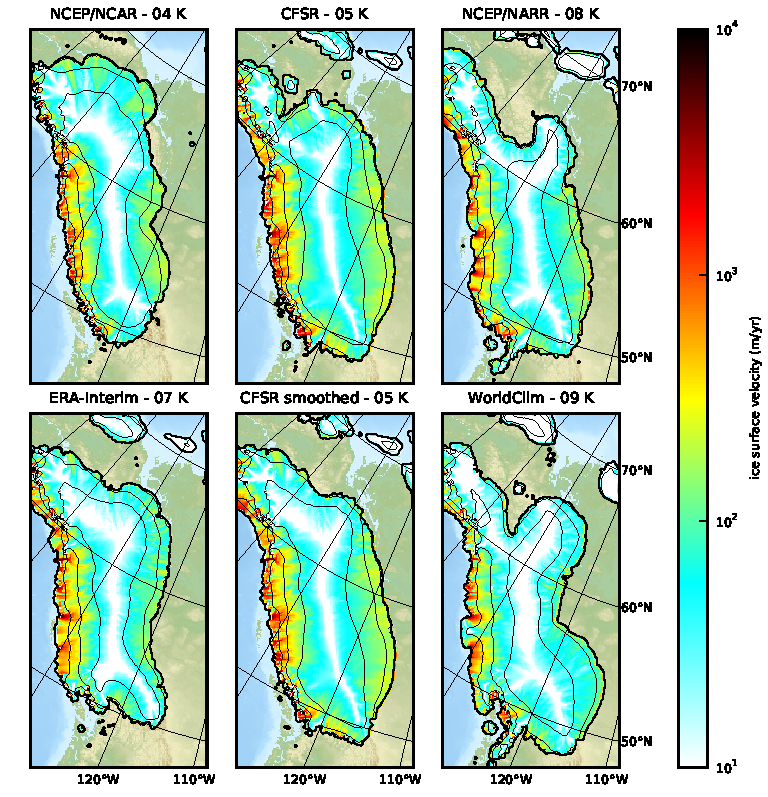
\includegraphics{cordillera-climate-best}
	\end{center}
	\caption{Ice surface topography (1\,km contours) after 10\,ka using temperature offsets resulting in glaciated areas of circa $2\,\times10^6\,\unit{km^2}$. A reconstructed LGM ice sheet margin by \citet{dyke-2004} (Fig.~\ref{fig:locmap}) is given for reference (blue line).}
	\label{fig:best}
\end{figure*}

% fig:durationstack
\begin{figure}[t]
	\vspace*{2mm}
	\begin{center}
		\includegraphics{cordillera-climate-durationstack}
	\end{center}
	\caption{Left panel: model sensitivity to simulation length. Modelled glaciated area, using NARR forcing data, and temperature offsets from 0 to 15\,\unit{\degree C}, solid lines corresponding to values from 7 to 11\,\unit{\degree C}. Right panel: modelled ice margin corresponding to temperature offsets from 7 to 11\,\unit{\degree C} when total glaciated area reach the approximate size of the LGM Cordilleran Ice Sheet of $2\,\times10^6\,\unit{km^2}$. A reconstructed LGM ice sheet margin by \citet{dyke-2004} (Fig.~\ref{fig:locmap}) is given for reference (grey shading). Note that shorter (and colder) simulations lead to more restrictive glaciation of the continental eastern margin but further ice extent in the maritime south-western part of the modelling domain.}
	\label{fig:durationstack}
\end{figure}
